\documentclass[11pt,a4paper]{article}

%% ---------------------------------------------------------------- packages
\usepackage[utf8]{inputenc}
\usepackage[T1]{fontenc}
\usepackage[english]{babel}
\usepackage[a4paper,margin=2.5cm]{geometry}
\usepackage{amsmath,amssymb}
\usepackage{siunitx}
\usepackage{booktabs}
\usepackage{graphicx}
\usepackage{caption}
\usepackage{subcaption}
\usepackage{enumitem}
\usepackage{xcolor}
\usepackage{wrapfig}
\usepackage{tikz}
\usetikzlibrary{arrows.meta,calc}
\usepackage[hidelinks]{hyperref}

\sisetup{detect-all, per-mode=symbol}
\captionsetup{font=small, labelfont=bf}
\setlength{\parindent}{0pt}
\setlength{\parskip}{0.6em}
\numberwithin{equation}{section}
\graphicspath{{figures/}}
\renewcommand{\topfraction}{0.9}
\renewcommand{\bottomfraction}{0.6}
\renewcommand{\textfraction}{0.07}
\renewcommand{\floatpagefraction}{0.85}

%% ---------------------------------------------------------------- shortcuts
\newcommand{\er}{\hat{\mathbf{e}}_r}
\newcommand{\ephi}{\hat{\mathbf{e}}_\phi}
\newcommand{\ii}{\hat{\boldsymbol{\imath}}}
\newcommand{\jj}{\hat{\boldsymbol{\jmath}}}
\newcommand{\kk}{\hat{\mathbf{k}}}
\newcommand{\vect}[1]{\mathbf{#1}}

\begin{document}

%% ================================================================ COVER
\begin{titlepage}
\centering
\vspace*{1.5cm}
\IfFileExists{logo_uc3m.png}{\includegraphics[width=4.2cm]{logo_uc3m.png}\\[1.2cm]}{\vspace*{1.5cm}}
{\Huge\scshape Universidad Carlos III de Madrid\par}
\vspace{0.4cm}
{\large Bachelor in Aerospace Engineering\par}
\vspace{1.2cm}
{\Large Mechanics Applied to Aerospace Engineering\par}
\vspace{0.8cm}
\rule{\linewidth}{1.2pt}\\[0.3cm]
{\LARGE\bfseries Particle Connected to a Spool\par}
\vspace{0.3cm}
\rule{\linewidth}{1.2pt}\\[0.8cm]
{\large Laboratory Session 1 --- Computer Session Report\par}
\vspace{1.2cm}
\begin{flushleft}
\hspace{1.2cm}\textit{Authors (Group LA):}\\
\hspace{1.2cm}Ismael Mart\'in D\'iez\\
\hspace{1.2cm}David Mart\'in Garc\'ia\\
\hspace{1.2cm}Alejandro Ranz Remart\'inez
\end{flushleft}
\vspace{1cm}
{\large\textbf{Report date:} October 9, 2026}
\vfill
\end{titlepage}

\tableofcontents
\newpage

%% ================================================================ 1 INTRODUCTION
\section{Introduction and Problem Statement}

A particle hanging from a string wound on a rotating spool has a moving constraint: the spool reels the string in, and the point where the string leaves the cylinder slides around it while the particle swings. The equations of motion are easy to write but cannot be integrated analytically in general, so in this session they are integrated numerically in MATLAB \cite{uc3m_guidelines,fernandez_lab1}.

We derive a tension-free equation for the single coordinate $\phi$ and integrate it with \texttt{ode45} for five study cases. The results are used to find when the mechanical energy is conserved and to explain the events of cases 3--5. At the end we discuss how the code should change to follow case 4 once the string goes slack.

\subsection{Problem Statement}

\begin{wrapfigure}{r}{0.47\textwidth}
\vspace{-1.2em}
\centering
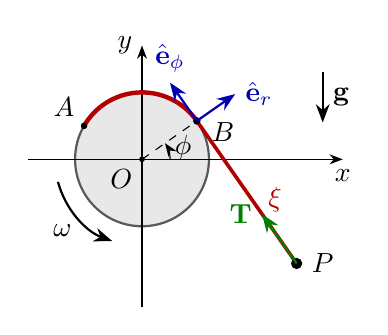
\begin{tikzpicture}[scale=0.85,>=Stealth]
  \coordinate (O) at (0,0);
  \coordinate (B) at (35:1);
  \coordinate (A) at (150:1);
  \coordinate (P) at ($(B)+(-55:2.6)$);
  \fill[gray!18] (O) circle (1);
  \draw[thick,gray!70!black] (O) circle (1);
  \draw[->] (-1.7,0) -- (3.0,0) node[below] {$x$};
  \draw[->] (0,-2.2) -- (0,1.7) node[left] {$y$};
  \draw[line width=1.6pt,red!70!black] (35:1) arc (35:150:1);
  \fill (A) circle (1.4pt) node[above left] {$A$};
  \draw[dashed] (O) -- (B);
  \draw[->] (0.42,0) arc (0:35:0.42);
  \node at (16:0.64) {$\phi$};
  \draw[->,thick] (195:1.3) arc (195:250:1.3);
  \node at (222:1.6) {$\omega$};
  \draw[line width=1.3pt,red!70!black] (B) -- (P) node[pos=0.55,right=2pt] {$\xi$};
  \fill (B) circle (1.6pt);
  \node[anchor=west] at ($(B)+(0.08,-0.16)$) {$B$};
  \fill (P) circle (2.4pt) node[right=2pt] {$P$};
  \fill (O) circle (1.2pt) node[below left] {$O$};
  \draw[->,thick,blue!70!black] (B) -- ++(35:0.7) node[right] {$\er$};
  \draw[->,thick,blue!70!black] (B) -- ++(125:0.7) node[above] {$\ephi$};
  \draw[->,thick] (2.7,1.3) -- (2.7,0.55) node[midway,right] {$\mathbf{g}$};
  \draw[->,thick,green!50!black] (P) -- ++(125:0.9) node[left] {$\mathbf{T}$};
\end{tikzpicture}
\caption{Spool, wrapped string (red arc from $B$ to the anchor $A$), polar basis at $B$ and tension on $P$.}
\label{fig:sketch}
\vspace{-1em}
\end{wrapfigure}

The particle $P$ has mass $m$ and hangs from a massless, inextensible string of total length $l$. The other end of the string is anchored at a point $A$ of a spool of radius $a$ and centre $O$, which turns counterclockwise at a constant rate $\omega$ (Fig.~\ref{fig:sketch}). $B$ is the point where the straight part of the string leaves the spool, at an angle $\phi$ from $Ox$, and $\xi$ is the length of the straight segment $BP$. The parameters are $g=\SI{9.81}{m/s^2}$, $m=\SI{0.1}{kg}$, $a=\SI{0.2}{m}$, $\phi(0)=0$ and $\xi(0)=\SI{1}{m}$; the five cases differ in $\omega$ and in the initial velocity $\dot x_P(0)$ (Table~\ref{tab:summary}).

\subsection{Degrees of Freedom and Constraint}

In the plane, $P$ needs two coordinates, and the pair $(\phi,\xi)$ is a valid choice through $\vect r_P=a\er-\xi\ephi$ (Eq.~\eqref{eq:pos}). The string removes one of them. The anchor $A$ is at the angle $\theta_A(t)=\theta_{A0}+\omega t$, the wrapped arc $BA$ has length $a(\theta_A-\phi)$, and the total length does not change:
\begin{equation}
  a\,(\theta_{A0}+\omega t-\phi) + \xi = l
  \quad\Longrightarrow\quad
  \xi(t,\phi) = \xi_0 - a\,(\omega t - \phi),
  \qquad \xi_0 = l - a\theta_{A0}. \label{eq:constraint}
\end{equation}
This is the same constraint as in the handwritten analytical solution. It has no velocities in it, so it is holonomic, and it contains $t$ explicitly through $\omega t$, so it is rheonomic. Therefore
\begin{equation}
  \text{C.D.O.F.} = 2 - 1 = 1,
\end{equation}
and $\phi(t)$ fixes the configuration once $t$ is known. With the chain rule,
\begin{equation}
  \dot\xi = \frac{\partial \xi}{\partial t} + \frac{\partial \xi}{\partial \phi}\,\dot\phi = a\dot\phi - a\omega. \label{eq:xidot}
\end{equation}
We assume that the string never unwinds completely ($\theta_A-\phi>0$); in case 4 this needs $l-\xi_0>\SI{0.254}{m}$.

\subsection{Reference Frame and Polar Basis}

The frame $Oxy$, with unit vectors $(\ii,\jj,\kk)$, is inertial, and every time derivative is taken in it. The vectors are projected on the polar basis attached to $B$:
\begin{equation}
  \begin{pmatrix}\er\\ \ephi\end{pmatrix} = [R(\phi)]\begin{pmatrix}\ii\\ \jj\end{pmatrix},\qquad
  [R(\phi)] = \begin{pmatrix}\cos\phi & \sin\phi\\ -\sin\phi & \cos\phi\end{pmatrix}.
\end{equation}
Since $\det R=\cos^2\phi+\sin^2\phi=1$ and $RR^{\mathsf T}=I$, $R$ is a rotation and its inverse is $R^{\mathsf T}$, which gives $\ii=\cos\phi\,\er-\sin\phi\,\ephi$ and $\jj=\sin\phi\,\er+\cos\phi\,\ephi$. The basis depends on $t$ only through $\phi$, so
\begin{equation}
  \dot{\hat{\mathbf e}}_r = \frac{d\er}{d\phi}\,\dot\phi = (-\sin\phi\,\ii+\cos\phi\,\jj)\,\dot\phi = \dot\phi\,\ephi,\qquad
  \dot{\hat{\mathbf e}}_\phi = \frac{d\ephi}{d\phi}\,\dot\phi = -(\cos\phi\,\ii+\sin\phi\,\jj)\,\dot\phi = -\dot\phi\,\er. \label{eq:basisdot}
\end{equation}

\subsection{Position, Velocity and Acceleration of \texorpdfstring{$P$}{P}}

$B$ lies on the spool, $\vect r_B=a\er$, and the string leaves it tangentially along $-\ephi$:
\begin{equation}
  \vect r_P = a\er - \xi\ephi
  \quad\Longleftrightarrow\quad
  x_P = a\cos\phi + \xi\sin\phi,\qquad y_P = a\sin\phi - \xi\cos\phi. \label{eq:pos}
\end{equation}
Differentiating with the product rule and using Eqs.~\eqref{eq:xidot} and \eqref{eq:basisdot}:
\begin{equation}
  \vect v_P = a\dot{\hat{\mathbf e}}_r - \dot\xi\,\ephi - \xi\dot{\hat{\mathbf e}}_\phi
  = a\dot\phi\,\ephi - (a\dot\phi-a\omega)\,\ephi + \xi\dot\phi\,\er
  \quad\Longrightarrow\quad
  \boxed{\vect v_P = \xi\dot\phi\,\er + a\omega\,\ephi}. \label{eq:vel}
\end{equation}
The two terms $a\dot\phi\,\ephi$ cancel, so the sliding of $B$ along the spool does not show up in the velocity of $P$. The component $\xi\dot\phi$ is the rotation of $BP$ about $B$, and $a\omega$, along the string, is the speed at which the spool reels the string in. Differentiating again, with $a$ and $\omega$ constant:
\begin{align}
  \vect a_P &= (\dot\xi\dot\phi + \xi\ddot\phi)\,\er + \xi\dot\phi\,\dot{\hat{\mathbf e}}_r + a\omega\,\dot{\hat{\mathbf e}}_\phi
  = \left[(a\dot\phi - a\omega)\dot\phi + \xi\ddot\phi - a\omega\dot\phi\right]\er + \xi\dot\phi^2\,\ephi \nonumber\\
  &\Longrightarrow\quad
  \boxed{\vect a_P = \left(a\dot\phi^2 + \xi\ddot\phi - 2a\omega\dot\phi\right)\er + \xi\dot\phi^2\,\ephi}. \label{eq:acc}
\end{align}
For $\omega=0$ the path is an involute of the circle with centre of curvature $B$, and $\xi\dot\phi^2$ is its centripetal acceleration.

%% ================================================================ 2 MODEL
\section{Mathematical Model and Dynamical Formulation}

\subsection{Forces on the Particle}

Two forces act on $P$: the tension, which pulls it towards $B$ ($T\geq0$, since a string cannot push), and its weight:
\begin{equation}
  \vect T = T\,\ephi;\qquad
  m\vect g = -mg\,\jj = -mg\left(\sin\phi\,\er + \cos\phi\,\ephi\right). \label{eq:forces}
\end{equation}

\subsection{Equation of Motion and String Tension}

Newton's second law in the inertial frame \cite{greenwood,meriam}, $m\vect a_P=\vect T+m\vect g$, projected on $\er$ and $\ephi$ with Eqs.~\eqref{eq:acc} and \eqref{eq:forces}:
\begin{align}
  \er:&\quad m\left(a\dot\phi^2 + \xi\ddot\phi - 2a\omega\dot\phi\right) = -mg\sin\phi, \label{eq:er}\\
  \ephi:&\quad m\xi\dot\phi^2 = T - mg\cos\phi. \label{eq:ephi}
\end{align}
$T$ only appears in Eq.~\eqref{eq:ephi}. Dividing Eq.~\eqref{eq:er} by $m\xi$ (valid while $\xi>0$) and substituting Eq.~\eqref{eq:constraint}:
\begin{equation}
  \boxed{\ddot\phi = \frac{-g\sin\phi - a\dot\phi^2 + 2a\omega\dot\phi}{\xi_0 - a(\omega t - \phi)}},\qquad
  \boxed{T(t,\phi,\dot\phi) = m\,\xi(t,\phi)\,\dot\phi^2 + mg\cos\phi}. \label{eq:eom}
\end{equation}
The equation is non-linear and depends on $t$ explicitly through $\xi(t,\phi)$. Dimensional check: $[g]=[a\dot\phi^2]=[a\omega\dot\phi]=\si{m/s^2}$, divided by $[\xi]=\si{m}$, gives $\si{s^{-2}}=[\ddot\phi]$, and $[m\xi\dot\phi^2]=[mg]=\si{kg.m/s^2}=\si{N}$.

%% ================================================================ 3 NUMERICS
\section{Numerical Implementation and State-Space Form}

\textbf{State-space form.} With $\vect X=[X_1,X_2]^{\mathsf T}=[\phi,\dot\phi]^{\mathsf T}$, Eq.~\eqref{eq:eom} becomes
\begin{equation}
  \frac{d\vect X}{dt} = \vect f(t,\vect X) =
  \begin{pmatrix} X_2 \\[2pt] \dfrac{-g\sin X_1 - aX_2^2 + 2a\omega X_2}{\xi_0 - a(\omega t - X_1)}\end{pmatrix}, \label{eq:ss}
\end{equation}
which is the local function \texttt{diffeq(t,X,g,omega,a,xi0)} of \texttt{main.m}. It is integrated with \texttt{ode45}, an embedded Runge--Kutta 4(5) method \cite{dormand_prince,shampine_reichelt}, with \texttt{RelTol}~$=$~\texttt{AbsTol}~$=10^{-8}$ and a maximum step of \SI{10}{ms}, so that every curve is sampled far above the Nyquist limit \cite{uc3m_guidelines}. The data give $\dot x_P(0)$, not $\dot\phi(0)$. At $\phi_0=0$ we have $\er=\ii$ and $\ephi=\jj$, so Eq.~\eqref{eq:vel} gives $\dot x_P(0)=\xi_0\dot\phi_0$ and $\dot\phi_0=\dot x_P(0)/\xi_0$; the vertical component $\dot y_P(0)=a\omega$ is set by the spool.

\textbf{Event function.} \texttt{stopfun} returns $\texttt{value}=[\xi-\xi_\mathrm{tol},\,T]$, $\texttt{isterminal}=[1,1]$ and $\texttt{direction}=[-1,-1]$, with $\xi$ and $T$ from Eqs.~\eqref{eq:constraint} and \eqref{eq:eom}. Near the spool $\ddot\phi\propto1/\xi$, and in a first run with $\xi_\mathrm{tol}=0$ \texttt{ode45} reduced its step to the minimum before reaching $\xi=0$ and stopped without reporting the event. The contact event is therefore placed at $\xi_\mathrm{tol}=\SI{e-6}{m}$, far below any real string thickness.

%% ================================================================ 4 RESULTS
\section{Simulation Results and Trajectories}

Table~\ref{tab:summary} summarises the five cases, and Figs.~\ref{fig:case1}--\ref{fig:case5} show $\phi(t)$, $\xi(t)$, $T(t)$ and the trajectory of $P$. Case 2 never triggers an event, so it is integrated over five periods.

\begin{table}[htbp]
\centering
\small
\caption{Study cases and main results. $t_\mathrm{end}$: time of the event (final time in case 2). Event $\xi=0$: the particle reaches the spool; $T=0$: the string goes slack.}
\label{tab:summary}
\begin{tabular}{@{}c S[table-format=1.1] S[table-format=-2.0] S[table-format=-1.5] S[table-format=2.5] c S[table-format=-1.5] S[table-format=-1.5] S[table-format=-1.5]@{}}
\toprule
Case & {$\omega$} & {$\dot x_P(0)$} & {$E_0$} & {$t_\mathrm{end}$} & Event & {$x_P(t_\mathrm{end})$} & {$y_P(t_\mathrm{end})$} & {$E(t_\mathrm{end})$}\\
 & {(rad/s)} & {(m/s)} & {(J)} & {(s)} & & {(m)} & {(m)} & {(J)}\\
\midrule
1 & 0.1 & 0   & -0.98098 & 50.00000 & $\xi=0$ & 0.20000  & 0.00000  & 0.00002\\
2 & 0   & -1  & -0.93100 & 10.00000 & none    & 0.29041  & -0.99593 & -0.93100\\
3 & 0   & -10 & 4.01900  & 0.27095  & $\xi=0$ & 0.05673  & 0.19178  & 4.01901\\
4 & 0   & 4   & -0.18100 & 1.69347  & $T=0$   & -0.68576 & -0.18966 & -0.18100\\
5 & 0.1 & 1   & -0.93098 & 35.50942 & $\xi=0$ & 0.02429  & -0.19852 & -0.19120\\
\bottomrule
\end{tabular}
\end{table}

\begin{figure}[tbp]
\centering
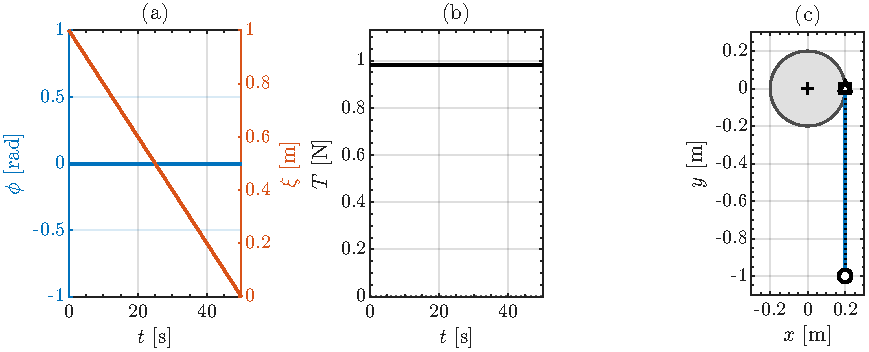
\includegraphics[width=0.85\textwidth]{fig_case1.pdf}
\caption{Case 1 ($\omega=\SI{0.1}{rad/s}$, $\dot x_P(0)=0$). (a) $\phi$ (left axis) and $\xi$ (right axis); (b) tension; (c) trajectory with the spool. $\circ$: initial position of $P$; $\triangle$: initial $B$; $\blacksquare$: final position. Dotted and dash-dotted lines: string at $t=0$ and at $t_\mathrm{end}$.}
\label{fig:case1}
\end{figure}

\begin{figure}[tbp]
\centering
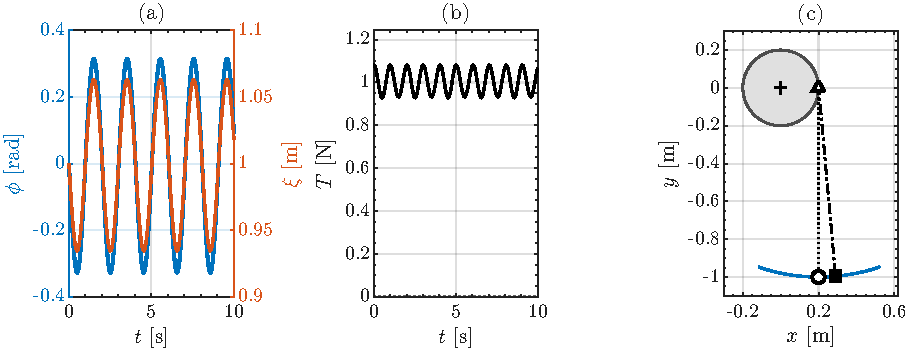
\includegraphics[width=0.85\textwidth]{fig_case2.pdf}
\caption{Case 2 ($\omega=0$, $\dot x_P(0)=\SI{-1}{m/s}$). Panels and markers as in Fig.~\ref{fig:case1}.}
\label{fig:case2}
\end{figure}

\begin{figure}[tbp]
\centering
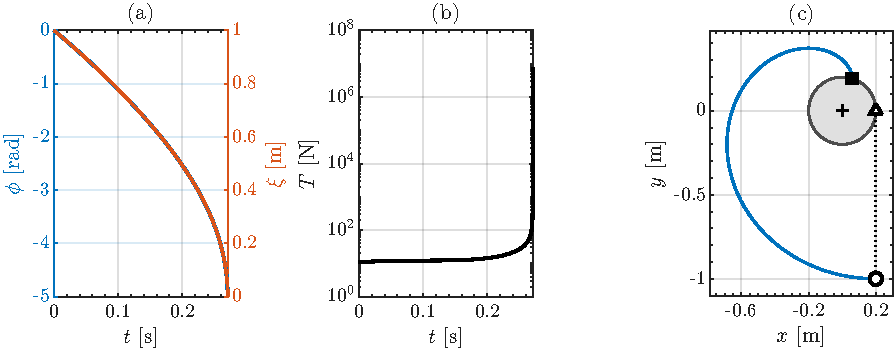
\includegraphics[width=0.85\textwidth]{fig_case3.pdf}
\caption{Case 3 ($\omega=0$, $\dot x_P(0)=\SI{-10}{m/s}$). With $\omega=0$, $\xi=\xi_0+a\phi$, so the two curves of (a) overlap on these scales. (b) is logarithmic.}
\label{fig:case3}
\end{figure}

\begin{figure}[tbp]
\centering
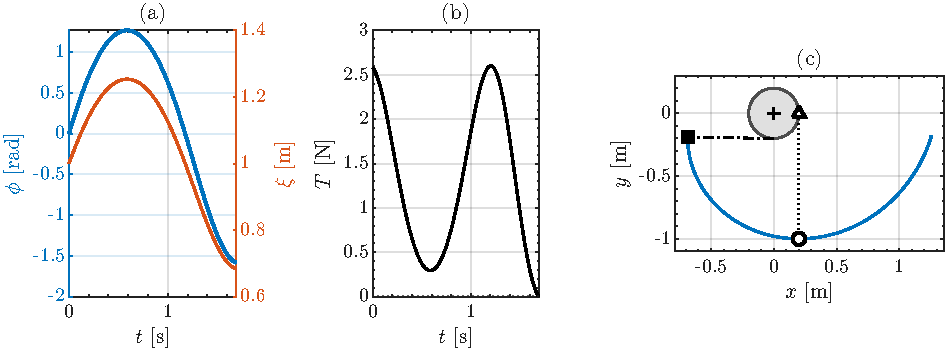
\includegraphics[width=0.85\textwidth]{fig_case4.pdf}
\caption{Case 4 ($\omega=0$, $\dot x_P(0)=\SI{4}{m/s}$). Panels and markers as in Fig.~\ref{fig:case1}.}
\label{fig:case4}
\end{figure}

\begin{figure}[tbp]
\centering
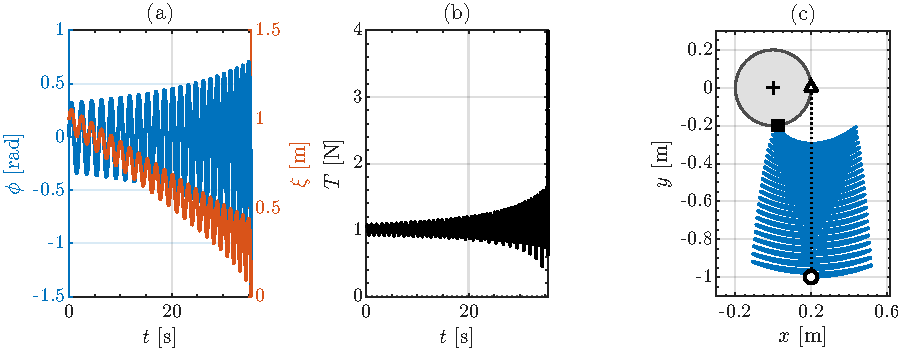
\includegraphics[width=0.85\textwidth]{fig_case5.pdf}
\caption{Case 5 ($\omega=\SI{0.1}{rad/s}$, $\dot x_P(0)=\SI{1}{m/s}$). (b) is cut at \SI{4}{N}; in the last milliseconds $T\simeq m|\vect v_P|^2/\xi$ grows without bound.}
\label{fig:case5}
\end{figure}

\textbf{Case 1.} With $\phi=\dot\phi=0$ the numerator of Eq.~\eqref{eq:ss} is zero for every $t$, so $\phi\equiv0$ is an exact solution. The spool works as a winch: $\xi=\xi_0-a\omega t$ drops linearly, $P$ rises vertically at $a\omega=\SI{0.02}{m/s}$, and since it does not accelerate, $T=mg=\SI{0.981}{N}$ (Fig.~\ref{fig:case1}). $P$ reaches the spool at $t=\xi_0/(a\omega)=\SI{50}{s}$, at $B=(a,0)$; the numerical solution keeps $\phi=0$ exactly.

\textbf{Case 2.} With the spool at rest, $\xi=\xi_0+a\phi$ is not constant: it oscillates between \num{0.93441} and \SI{1.06282}{m} as the string wraps and unwraps (Fig.~\ref{fig:case2}). The swing is not symmetric. $\phi$ goes from \SI{-0.32795}{rad} to \SI{0.31409}{rad}, because both turning points are at the same height (energy is conserved) while the pivot $B$ moves with $\phi$. The tension stays between \num{0.929} and \SI{1.081}{N}, so no event occurs and the motion is periodic.

\textbf{Case 3.} The fast launch to the left wraps the string clockwise around the spool. $\phi$ decreases monotonically to \SI{-5}{rad} (\SI{-286.5}{\degree}), where $\xi=\xi_0+a\phi=0$, and the path spirals in (Fig.~\ref{fig:case3}c). The tension starts at $m\dot x_P(0)^2/\xi_0+mg=\SI{10.98}{N}$ and grows without bound before contact (Fig.~\ref{fig:case3}b).

\textbf{Case 4.} $P$ first swings to the right, unwinds string up to $\xi=\SI{1.2533}{m}$ and turns back at $\phi_\mathrm{max}=\SI{1.26667}{rad}$, below $\pi/2$. It then passes the lowest point and rises on the left, where part of the string is wrapped, until the tension vanishes at $t=\SI{1.69347}{s}$ (Fig.~\ref{fig:case4}).

\textbf{Case 5.} This case adds the oscillation of case 2 to the winding of case 1. As the string gets shorter the oscillation speeds up and its amplitude grows from $|\phi|\simeq\SI{0.32}{rad}$ to about \SI{0.73}{rad}. The tension oscillates around a slowly rising mean and stays positive (Fig.~\ref{fig:case5}b).

%% ================================================================ 5 DISCUSSION
\section{Physical Discussion and Energy}

\subsection{Mechanical Energy}

The mechanical energy of $P$, with $V=mgy_P$ and $|\vect v_P|^2=\xi^2\dot\phi^2+a^2\omega^2$ from Eq.~\eqref{eq:vel}, is
\begin{equation}
  E = \tfrac12 m\left(\xi^2\dot\phi^2 + a^2\omega^2\right) + mg\left(a\sin\phi - \xi\cos\phi\right). \label{eq:energy}
\end{equation}
By the work--energy theorem $dK/dt=(\vect T+m\vect g)\cdot\vect v_P$, and the weight is conservative, $m\vect g\cdot\vect v_P=-dV/dt$. Only the power of the tension is left:
\begin{equation}
  \frac{dE}{dt} = \vect T\cdot\vect v_P = T\,\ephi\cdot\left(\xi\dot\phi\,\er + a\omega\,\ephi\right) = Ta\omega. \label{eq:power}
\end{equation}
While the string is taut $T>0$, so $E$ is conserved if and only if $\omega=0$ (cases 2--4). For $\omega>0$ (cases 1 and 5) $E$ increases all the time: the motor that turns the spool reels the string in at speed $a\omega$ against the tension, and that work goes into $P$.

\begin{figure}[tbp]
\centering
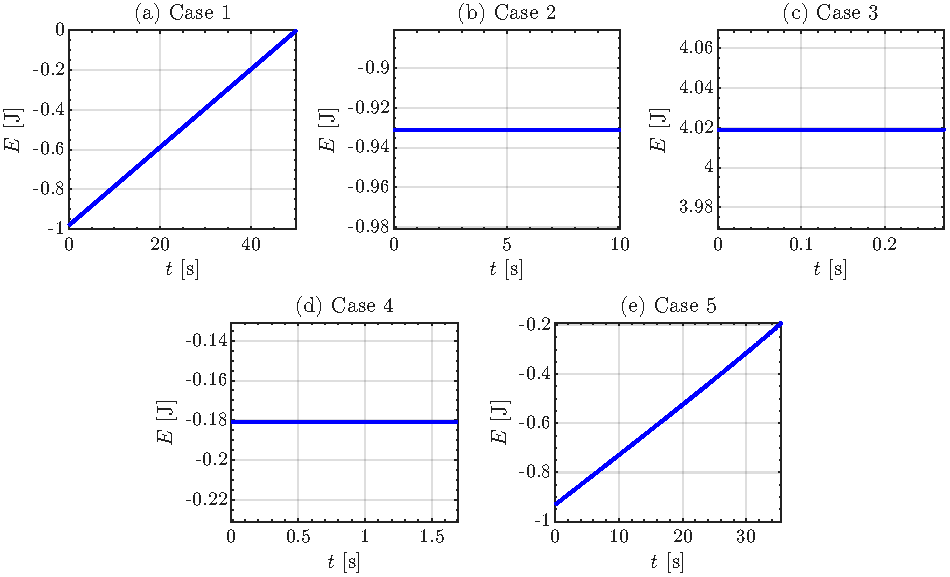
\includegraphics[width=0.8\textwidth]{fig_energy.pdf}
\caption{Mechanical energy of each case, Eq.~\eqref{eq:energy}. For $\omega=0$ the vertical axis spans $E_0\pm\SI{0.05}{J}$.}
\label{fig:energy}
\end{figure}

Fig.~\ref{fig:energy} agrees with Eq.~\eqref{eq:power}. In cases 2--4 $E$ stays at $E_0$, since the tension is perpendicular to $\vect v_P=\xi\dot\phi\,\er$ and does no work. In cases 1 and 5 $E$ grows. In case 1, $T=mg$ and $E=E_0+mga\omega t$ rises linearly from \SI{-0.98098}{J} to \SI{0.00002}{J}; in case 5 it rises from \SI{-0.93098}{J} to \SI{-0.19120}{J}, slightly faster than in case 1 because the swing adds $m\xi\dot\phi^2$ to the tension.

\subsection{Critical Events}\label{sec:critical}

\textbf{Case 3: contact with the spool.} The particle hits the spool at $t_c=\SI{0.270947}{s}$, with $\phi_c=\SI{-5.00000}{rad}$ and $\vect r_P(t_c)=\vect r_B=a\er(\phi_c)=(\num{0.05673},\,\num{0.19178})$~\si{m}, in the upper-right quadrant after wrapping \SI{286.5}{\degree} of string. With $\omega=0$ the energy is conserved, so the speed $|\vect v_P|=\xi|\dot\phi|=\sqrt{2(E_0/m-gy_P)}$ stays finite, and at contact it is $v_c=\SI{8.7531}{m/s}$. Then
\begin{equation}
  |\dot\phi| = \frac{|\vect v_P|}{\xi} \simeq \frac{v_c}{\xi} \xrightarrow[\xi\to0]{}\infty, \label{eq:sing}
\end{equation}
so near the end $\dot\phi$ grows like $1/\xi$ (Fig.~\ref{fig:phidot}) while the speed of $P$ stays finite. The tension $T\simeq mv_c^2/\xi$ diverges as well.

\begin{figure}[tbp]
\centering
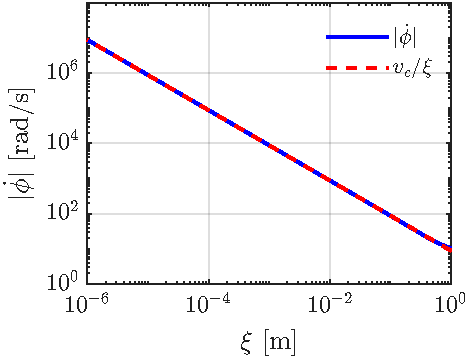
\includegraphics[width=0.45\textwidth]{fig_case3_phidot.pdf}
\caption{Case 3: $|\dot\phi|$ against $\xi$ near the contact, compared with $v_c/\xi$ from Eq.~\eqref{eq:sing}.}
\label{fig:phidot}
\end{figure}

\textbf{Case 4: loss of tension.} From Eq.~\eqref{eq:eom}, $T=0$ means $m\xi\dot\phi^2=-mg\cos\phi$, which needs $\cos\phi<0$. So the string can only go slack when $BP$ points above the horizontal line through $B$, where the inward part of the weight can be larger than the centripetal force that keeps $P$ on its arc. On the right swing $\phi_\mathrm{max}<\pi/2$ and this never happens. On the left, the wrapped string is shorter and $B$ drops to $y\simeq\SI{-0.2}{m}$, so $P$, with the same energy, rises above the horizontal through $B$. The tension vanishes at $t_s=\SI{1.69347}{s}$, with $\phi_s=\SI{-1.58590}{rad}$, $\xi_s=\SI{0.68282}{m}$, $\vect r_P(t_s)=(\num{-0.68576},\,\num{-0.18966})$~\si{m} and $|\vect v_P|=\SI{0.318}{m/s}$; indeed $\xi_s\dot\phi_s^2=\SI{0.148}{m/s^2}=g|\cos\phi_s|$.

\textbf{Case 5: stop condition.} The tension never vanishes ($\min T=\SI{0.455}{N}$), so the stop condition is contact with the spool, $\xi=0$, at $t=\SI{35.50942}{s}$ and $\vect r_P=(\num{0.02429},\num{-0.19852})$~\si{m}, near the bottom of the spool. By Eq.~\eqref{eq:constraint}, contact happens when $\omega t-\phi=\xi_0/a=\SI{5}{rad}$. The winding gives $\omega t=\SI{3.551}{rad}$ and a swing to the left ($\phi=\SI{-1.449}{rad}$) wraps the rest, so contact comes \SI{14.5}{s} earlier than in case 1.

%% ================================================================ 6 SLACK
\section{Motion After the Loss of Tension}\label{sec:slack}

After $t_s$ the string cannot push, Eq.~\eqref{eq:constraint} no longer holds and $P$ has two degrees of freedom again, so \texttt{diffeq} is no longer valid. To keep integrating case 4, the code would need these changes:
\begin{enumerate}[leftmargin=1.5em, itemsep=0.2em]
  \item \textbf{A second model.} When \texttt{stopfun} detects $T=0$, the integration switches to free flight under gravity, $\ddot x_P=0$ and $\ddot y_P=-g$, with a new state vector $\vect Y=[x_P,y_P,\dot x_P,\dot y_P]^{\mathsf T}$ and a new function for $d\vect Y/dt$.
  \item \textbf{Initial conditions at the switch.} Position and velocity are continuous at $t_s$, so the flight starts from $\vect r_P(t_s)$ and $\vect v_P(t_s)$ given by Eqs.~\eqref{eq:pos} and \eqref{eq:vel}.
  \item \textbf{A new event function.} During the flight the string is slack while $P$ is closer to the spool than the string allows. With $\omega=0$ the wrapped part does not move, so the string becomes taut again when $|\vect r_P-\vect r_B(\phi_s)|=\xi_s$. A second event, $|\vect r_P|=a$, would detect if $P$ hits the spool.
  \item \textbf{Back to the constrained model.} When the string becomes taut, it pulls $P$ with an impulse that removes the velocity component along the string. The integration with \texttt{diffeq} and \texttt{stopfun} restarts from the new $\phi$ and $\dot\phi=\vect v_P\cdot\er/\xi$, and the two models alternate in a loop until the final time.
\end{enumerate}

%% ================================================================ 7 CONCLUSIONS
\section{Conclusions}

\begin{itemize}[leftmargin=1.5em, itemsep=0.3em]
  \item The particle has one degree of freedom, $\phi$, with the holonomic, rheonomic constraint $\xi=\xi_0-a(\omega t-\phi)$; Newton's law gives a tension-free equation for $\ddot\phi$ and an explicit $T(t,\phi,\dot\phi)$.
  \item $\dot E=Ta\omega$: the energy is conserved only with the spool at rest (cases 2--4) and grows whenever the spool reels the string in (cases 1 and 5).
  \item In case 3 the particle hits the spool at $t=\SI{0.27095}{s}$, at $(\num{0.05673},\num{0.19178})$~\si{m}, and $\dot\phi$ grows like $1/\xi$ while the speed stays finite. In case 4 the string goes slack at $t=\SI{1.69347}{s}$, once $BP$ rises above the horizontal through $B$. Case 5 stops by contact with the spool at $t=\SI{35.50942}{s}$.
  \item Following case 4 after $T=0$ needs a second, free-flight model and an event that detects when the string becomes taut again.
\end{itemize}
The problem reduces to one ODE in $\phi$, and only the rotation of the spool can change the mechanical energy of $P$.

%% ================================================================ REFERENCES
\phantomsection
\addcontentsline{toc}{section}{References}
{\footnotesize
\bibliographystyle{unsrt}
\bibliography{references}}

\end{document}
